\documentclass[tikz,border=3.14mm]{standalone}
\usepackage{pgfplots}
\pgfplotsset{compat=1.18}

\begin{document}

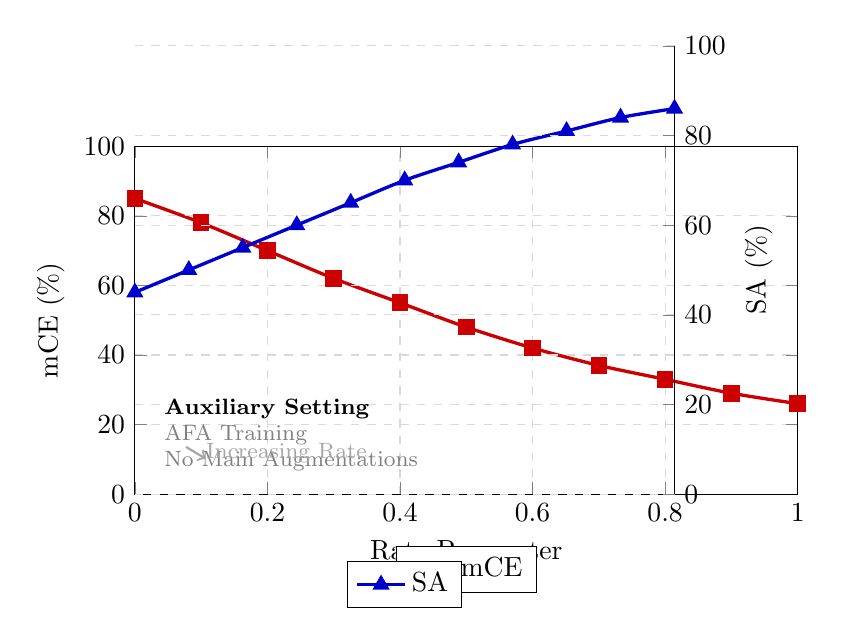
\begin{tikzpicture}
  \begin{axis}[
    width=10cm,
    height=6cm,
    xlabel={Rate Parameter},
    ylabel={mCE (\%)},
    ymin=0, ymax=100,
    xmin=0, xmax=1,
    grid=both,
    grid style={dashed, gray!30},
    legend style={at={(0.5,-0.15)}, anchor=north, legend columns=2},
    axis on top
  ]
  \addplot[
    color=red!80!black,
    mark=square*,
    mark options={fill=red!80!black, scale=1.2},
    line width=1.2pt,
    smooth
  ] coordinates {
    (0.0, 85) (0.1, 78) (0.2, 70) (0.3, 62) (0.4, 55) (0.5, 48) (0.6, 42) (0.7, 37) (0.8, 33) (0.9, 29) (1.0, 26)
  };
  \addlegendentry{mCE}
  
  \end{axis}
  
  \begin{axis}[
    ylabel={SA (\%)},
    ymin=0, ymax=100,
    xmin=0, xmax=1,
    axis y line*=right,
    axis x line=none,
    grid=both,
    grid style={dashed, gray!30},
    legend style={at={(0.5,-0.15)}, anchor=north, legend columns=2},
    axis on top
  ]
  \addplot[
    color=blue!80!black,
    mark=triangle*,
    mark options={fill=blue!80!black, scale=1.2},
    line width=1.2pt,
    smooth
  ] coordinates {
    (0.0, 45) (0.1, 50) (0.2, 55) (0.3, 60) (0.4, 65) (0.5, 70) (0.6, 74) (0.7, 78) (0.8, 81) (0.9, 84) (1.0, 86)
  };
  \addlegendentry{SA}
  
  \end{axis}
  
  % Annotations
  \node[anchor=west, align=left, font=\footnotesize] at (0.25, 0.75) {
    \textbf{Auxiliary Setting} \\
    \textcolor{gray}{AFA Training} \\
    \textcolor{gray}{No Main Augmentations}
  };
  
  \draw[->, thick, gray!70] (0.65, 0.6) -- (0.9, 0.45) node[midway, right, font=\footnotesize, gray!70] {Increasing Rate};
\end{tikzpicture}

\end{document}